% Document Preamble
\documentclass[11pt]{beamer}

\usepackage{amsmath}
\usepackage{multimedia}
%\usepackage[activeacute,english]{babel}
%\usepackage[latin1]{inputenc}
%\usepackage{xcolor}
%\usepackage[percent]{overpic}
%\usepackage{dcolumn}
%\usepackage{booktabs}
%\usepackage[absolute,overlay]{textpos}
%\usepackage{tikz}
%\usepackage{amsfonts}
%\usepackage{amssymb}
%\usepackage{makeidx}

\usepackage{anyfontsize}
\usefonttheme[onlymath]{serif}  %  Use this for sans-serif text and proper tex math, in italic serif (thanks to Max Floetotto for this)
\usefonttheme{structuresmallcapsserif} % Titles will appear in Small Cap Serif

% -----------------------------------------
% Center the Frame Title
% -----------------------------------------

\setbeamertemplate{frametitle} {
\begin{centering}
\vspace{0.1in} \insertframetitle
\par
\end{centering}}
\setbeamercolor{frametitle}{fg=black!50!blue}
\setbeamercolor{title}{fg=black!50!blue}
\setbeamercolor{button}{bg=black!50!gray,fg=white}


% -----------------------------------------
% Number the slides but don't show the distracting total number of slides
% -----------------------------------------

\setbeamertemplate{footline}{\hspace{350pt}\insertframenumber \vspace{0.1in}}  %  Thanks to Jihee Kim for figuring out how to suppress the total number of slides

% -----------------------------------------
% Get rid of the irritating navigation bar
% -----------------------------------------

\setbeamertemplate{navigation symbols}{}


\begin{document}

\title{Discussion 1: \\ Differential and Difference Equations - Theory}
\author{Stefano Pica \\ Boston University}
\date{September 6, 2019}

%%%%%%%%%%%%%%%%%%%%%%%
%%%%%%%% FRAME %%%%%%%%
%%%%%%%%%%%%%%%%%%%%%%%

\begin{frame}
	\titlepage
\end{frame}

%%%%%%%%%%%%%%%%%%%%%%%
%%%%%%%% FRAME %%%%%%%%
%%%%%%%%%%%%%%%%%%%%%%%

\begin{frame}
\frametitle{Introduction}
\begin{itemize}\itemsep2ex
	\item Economists need to know basic theory of difference and differential equations as they describe law of motions of variables of interest
	\item Differential equations describe movements in continuous time, difference equations in discrete time
	\item Reference on differential equations: Acemoglu, Introduction to Modern Economic Growth. Appendix B
	\item Reference on difference equations: Galor, Dynamical Systems
	\item If you find any typos in these or future slides, please send me an email so I can correct them
\end{itemize}
\end{frame}

%%%%%%%%%%%%%%%%%%%%%%%
%%%%%%%% FRAME %%%%%%%%
%%%%%%%%%%%%%%%%%%%%%%%

\begin{frame}
	\frametitle{Outline}
	\tableofcontents
\end{frame}

%%%%%%%%%%%%%%%%%%%%%%%%%%%%%%%
%%%%%%%%%%% SECTION %%%%%%%%%%%
%%%%%%%%%%%%%%%%%%%%%%%%%%%%%%%

\section{Differential Equations and Stability}

%%%%%%%%%%%%%%%%%%%%%%%
%%%%%%%% FRAME %%%%%%%%
%%%%%%%%%%%%%%%%%%%%%%%

\begin{frame}
\frametitle{Some Terminology}
\begin{itemize}\itemsep2ex
	\item An explicit first order differential equation (DE) is
	\begin{equation}
	\label{DE1}
	\frac{dx(t)}{dt} \equiv \dot{x(t)} = g(x(t),t)
	\end{equation}
	\item An implicit first order DE is
	\begin{equation*}
	H(\dot{x(t)},x(t),t) = 0
	\end{equation*}
	\item We will deal only with first-order explicit DEs.
	\item A DE is \textit{autonomous} if it can be written as
	\begin{equation*}
	\dot{x(t)} = g(x(t))
	\end{equation*}
\end{itemize}
\end{frame}

%%%%%%%%%%%%%%%%%%%%%%%
%%%%%%%% FRAME %%%%%%%%
%%%%%%%%%%%%%%%%%%%%%%%

\begin{frame}
\frametitle{Some Terminology}
\begin{itemize}\itemsep2ex
	\item An nth-order DE is
	\begin{equation*}
	\frac{d^nx(t)}{dt^n} = g \left (\frac{d^{n-1}x(t)}{dt^{n-1}},\dots,\frac{dx(t)}{dt},x(t),t \right)
	\end{equation*}
	\item Higher order DE can always be transformed to systems of first-order DEs
	\item A linear first-order DE takes the form
	\begin{equation*}
	\dot{x(t)} = a(t) x(t) + b(t)
	\end{equation*}
	\item \textit{Homogenous equation}: $b(t)=0$.
	\item \textit{Constant coefficient equation}: $a(t)=a$, $b(t)=b$.
\end{itemize}
\end{frame}

%%%%%%%%%%%%%%%%%%%%%%%
%%%%%%%% FRAME %%%%%%%%
%%%%%%%%%%%%%%%%%%%%%%%

\begin{frame}
\frametitle{Initial Value Problem}
\begin{itemize}\itemsep2ex
	\item In economics, a \textit{state variable} is a variable which is backward looking (e.g. a stock of capital). In this case, a differential equation as in \eqref{DE1} is specified together with an initial condition $x(0)=x_0$.
	\item \textbf{Example}: Assume capital $k$ evolves each period by a factor $a>1$, and consider the initial condition $k(0)=k_0$.
	\begin{equation*}
	\dot{k(t)} = a k(t)
	\end{equation*}
	Divide both sides by $k(t)$ and integrate wrt $t$ to get
	\begin{equation*}
	\ln |k(t)| + c_0 = a t + c_1
	\end{equation*}
	Take exponent on both sides to get the \textit{general solution}
	\begin{equation*}
	k(t) = c \exp(a t)
	\end{equation*}
	Plug initial condition to get $k(t) = k_0 \exp(a t)$.
\end{itemize}
\end{frame}

%%%%%%%%%%%%%%%%%%%%%%%
%%%%%%%% FRAME %%%%%%%%
%%%%%%%%%%%%%%%%%%%%%%%

\begin{frame}
\frametitle{Terminal condition}
\begin{itemize}\itemsep2ex
	\item A \textit{co-state variable} is a variable which instead depends on the future (e.g. prices, value functions, marginal utilities). In this case, boundary conditions are specified by ``transversality conditions'': the terminal value of $x(t)$ is specified at some $T<\infty$ or $T=\infty$.
	\item Will soon see examples of transversality condition in this course.
	% \item \textbf{Example}: Consider the following homogenous linear DE without constant coefficients $\dot{x(t)} = a(t) x(t)$
	% Divide both sides by $x(t)$, integrate wrt $t$ and take exponent
	% \begin{equation*}
	% x(t) = c \exp \left( \int_0^t a(s) ds \right )
	% \end{equation*}
	% With terminal condition $x(T)=x_T$: $c = x_T / \exp \left( \int_0^T a(s) ds \right )$ and so
	% \begin{equation*}
	% x(t) = x_T \exp \left( \int_0^t a(s) ds - \int_0^T a(s) ds \right )
	 %\end{equation*}
\end{itemize}
\end{frame}

%%%%%%%%%%%%%%%%%%%%%%%
%%%%%%%% FRAME %%%%%%%%
%%%%%%%%%%%%%%%%%%%%%%%

\begin{frame}
\frametitle{General versus Particular Solution}
\begin{itemize}\itemsep2ex
	\item Go back to
	\begin{equation*}
	\dot{x(t)} = g(x(t),t)
	\end{equation*}
	\item A family of functions that satisfies the previous equation is called a ``general solution''
	\item Furthermore, if a boundary condition is specified, then the function that solves the differential equation and satisfies the boundary condition is called ``particular solution''.
	\item The boundary condition pins down the constant in the solution. See previous slides.
\end{itemize}
\end{frame}

%%%%%%%%%%%%%%%%%%%%%%%
%%%%%%%% FRAME %%%%%%%%
%%%%%%%%%%%%%%%%%%%%%%%

\begin{frame}
\frametitle{Solving a Non-Homogenous Linear DE with Constant Coefficients}
\begin{itemize}\itemsep2ex
	\item Start from
	\begin{equation}
	\label{nonhomoconst}
	\dot{x(t)} = a x(t) + b
	\end{equation}
	\item Let $y(t) = x(t) + b/a$. Then rewrite \eqref{nonhomoconst} as
	\begin{equation*}
	\dot{y(t)} = a y(t)
	\end{equation*}
	\item Solve it as previous case to get $y(t) = c \exp(a t)$, then change the variable back
	\begin{equation*}
	x(t) = -b/a + c \exp(a t)
	\end{equation*}
	\item With initial condition $x(0)=x_0$: $c = x_0 + b/a$.
\end{itemize}
\end{frame}

%%%%%%%%%%%%%%%%%%%%%%%
%%%%%%%% FRAME %%%%%%%%
%%%%%%%%%%%%%%%%%%%%%%%

\begin{frame}
\frametitle{Solving a Non-Homogenous Linear DE with Constant Coefficients}
\begin{itemize}\itemsep2ex
	\item Therefore the particular solution is
	\begin{equation*}
	x(t) = -b/a + (x_0 + b/a) \exp(a t)
	\end{equation*}
	\item Let's discuss \textbf{stability}. Steady state, where $\dot{x(t)}=0$, is
	\begin{equation*}
	x(t) = x^* = - b/a
	\end{equation*}
	\item Two cases as t increases
	\begin{itemize}\itemsep2ex
		\item $a<0$: $x(t)$ apporaches $x^*$
		\item $a>0$: $x(t)$ diverges
	\end{itemize}
\end{itemize}
\end{frame}

%%%%%%%%%%%%%%%%%%%%%%%
%%%%%%%% FRAME %%%%%%%%
%%%%%%%%%%%%%%%%%%%%%%%

\begin{frame}
\frametitle{Systems of Linear Differential Equations}
\begin{itemize}\itemsep2ex
	\item Consider a system of first-order DEs with constant coefficients
	\begin{equation}
	\label{systemdiff}
	\dot{x(t)} = A x(t)
	\end{equation}
	\item This system always has a unique solution
	\item \textbf{Theorem}: Suppose A has n distinct real eigenvalues $\xi_1, \dots, \xi_n$. Then the unique solution to the system \eqref{systemdiff} takes the form
	\begin{equation*}
	x(t) = \sum_{j=1}^n c_j \exp(\xi_j t) v_{\xi_j}
	\end{equation*}
	 where $v_{\xi_1}, \dots, v_{\xi_n}$ denote the eigenvectors corresponding to the
	 eigenvalues $\xi_1, \dots, \xi_n$, and $c_1, \dots, c_n$ denote the constants of integration
	\item Note: the constant of integration are determined by the boundary conditions.
\end{itemize}
\end{frame}

%%%%%%%%%%%%%%%%%%%%%%%
%%%%%%%% FRAME %%%%%%%%
%%%%%%%%%%%%%%%%%%%%%%%

\begin{frame}
\frametitle{Stability}
\begin{itemize}\itemsep2ex
	\item The stability properties of the system depend on the signs of its eigenvalues.
	\begin{itemize}\itemsep2.5ex
		\item If all eigenvalues are positive, the system is unstable
		\item If $m<n$ eigenvalues are negative, then there exists an m-dimensional subspace such that the solution tends to the steady state only starting with an initial value on this subspace (\textit{saddle path stability})
		\item If eigenvalues are complex, the system entails oscillating behaviour
		\item The system is stable only when all eigenvalues are negative
	\end{itemize}
\end{itemize}
\end{frame}

%%%%%%%%%%%%%%%%%%%%%%%%%%%%%%%
%%%%%%%%%%% SECTION %%%%%%%%%%%
%%%%%%%%%%%%%%%%%%%%%%%%%%%%%%%

\section{Difference Equations and Stability}

%%%%%%%%%%%%%%%%%%%%%%%
%%%%%%%% FRAME %%%%%%%%
%%%%%%%%%%%%%%%%%%%%%%%

\frame{\tableofcontents[currentsection,hideothersubsections,currentsubsection]}

%%%%%%%%%%%%%%%%%%%%%%%
%%%%%%%% FRAME %%%%%%%%
%%%%%%%%%%%%%%%%%%%%%%%

\begin{frame}
\frametitle{Linear Systems and Solution}
\begin{itemize}\itemsep2ex
	\item One-dimensional, first-order, autonomous, linear difference equation
	\begin{equation}
	\label{D1}
	y_{t+1} = a y_t + b
	\end{equation}
	\item A solution to \eqref{D1} is a trajectory of the state variable $(y_t)_{t=0}^{\infty}$ that satisfies the law of motion at any point in time.
	\item The derivation may follow several methods, we'll use ``method of iterations''.
	\item Given an initial value $y_0$, start at time 1 $y_1 = a y_0 + b$ and substitute recursively to get
	\begin{equation*}
	y_{t} = a^t y_0 + b \sum_{i=0}^{t-1} a^i
	\end{equation*}
\end{itemize}
\end{frame}

%%%%%%%%%%%%%%%%%%%%%%%
%%%%%%%% FRAME %%%%%%%%
%%%%%%%%%%%%%%%%%%%%%%%

\begin{frame}
\frametitle{Linear Systems and Solution}
\begin{itemize}\itemsep2ex
	\item $\sum_{i=0}^{t-1} a^i$ is a geometric series with factor $a$, so
	\[\sum_{i=0}^{t-1} a^i =   \left\{
	\begin{array}{ll}
     \frac{1-a^t}{1-a} & \text{if} \hspace{0.3cm}a \neq 1 \\
     t & \text{if} \hspace{0.3cm} a = 1 \\
	\end{array}
	\right. \]
	and therefore
	\[y_t =   \left\{
	\begin{array}{ll}
   	a^t y_0 + b \frac{1-a^t}{1-a} & \text{if} \hspace{0.3cm} a \neq 1 \\
   	y_0 + b t & \text{if} \hspace{0.3cm}  a = 1 \\
	\end{array}
	\right. \]
 	or alternatively
 	\[y_t =   \left\{
	\begin{array}{ll}
   	[y_0-\frac{b}{1-a}] a^t + \frac{b}{1-a} & \text{if} \hspace{0.3cm} a \neq 1 \\
   	y_0 + b t & \text{if} \hspace{0.3cm}  a = 1 \\
	\end{array}
	\right. \]
	\item Thus the entire trajectory of the state variable is uniqued determined given the initial condition
\end{itemize}
\end{frame}

%%%%%%%%%%%%%%%%%%%%%%%
%%%%%%%% FRAME %%%%%%%%
%%%%%%%%%%%%%%%%%%%%%%%

\begin{frame}
\frametitle{Existence and Uniqueness of Steady-State Equilibria}
\begin{itemize}\itemsep2ex
	\item A steady state equilibrium (SS) of the difference equation $y_{t+1} = a y_t + b$ is $\bar{y}$ such that $\bar{y} = a \bar{y} + b$
	\item A SS exists if and only if $a \neq 1$ or $\{a=1$ and $b=0\}$:
	\[\bar{y} =   \left\{
	\begin{array}{ll}
    \frac{b}{1-a} & \text{if} \hspace{0.3cm} a \neq 1 \\
   	y_0 & \text{if} \hspace{0.3cm}  a = 1 \hspace{0.3cm} \text{and} \hspace{0.3cm} b=0  \\
	\end{array}
	\right. \]
	\item Finally, the SS is unique if and only if $a \neq 1$ (the second case entail a continuum of SS reflecting the entire set of feasible initial conditions)
	\item Therefore substituting the value of $\bar{y}$ into the solution previously found

 	\[y_t =   \left\{
	\begin{array}{ll}
    [y_0-\bar{y}] a^t + \bar{y} & \text{if} \hspace{0.3cm} a \neq 1 \\
    y_0 + b t & \text{if} \hspace{0.3cm}  a = 1 \\
	\end{array}
	\right. \]
\end{itemize}
\end{frame}

%%%%%%%%%%%%%%%%%%%%%%%
%%%%%%%% FRAME %%%%%%%%
%%%%%%%%%%%%%%%%%%%%%%%

\begin{frame}
\frametitle{Stability of Steady-State Equilibria}
\begin{itemize}\itemsep2ex
	\item A steady state equilibrium $\bar{y}$ of the difference equation $y_{t+1} = a y_t + b$ is
	\begin{itemize}\itemsep2ex
		\item globally (asymptotically) stable if $\lim_{t \to \infty} y_t = \bar{y}  \hspace{0.2cm} \forall y_0$
		\item locally (asymptotically) stable if $\lim_{t \to \infty} y_t = \bar{y}  \hspace{0.2cm} \forall y_0$ such that $|y_0 - \bar{y}| < \epsilon$ for some $\epsilon>0$
	\end{itemize}
	\item A steady state equilibrium $\bar{y}$ of the difference equation $y_{t+1} = a y_t + b$ is globally asymptotically stable only if it is unique
	\begin{itemize}\itemsep2ex
		\item While global stability requires global uniqueness of the SS, local stability necessitates the local uniqueness of the SS
	\end{itemize}
\end{itemize}
\end{frame}

%%%%%%%%%%%%%%%%%%%%%%%
%%%%%%%% FRAME %%%%%%%%
%%%%%%%%%%%%%%%%%%%%%%%

\begin{frame}
\frametitle{Stability of Steady-State Equilibria}
\begin{itemize}\itemsep2ex
	\item As follows from the definition of stability, we have to examine the system as time approaches infinity. This leads to
	\[
	\lim_{t \to \infty} |y_t| =   \left\{
	\begin{array}{ll}
    |\bar{y}| & \text{if} \hspace{0.3cm} |a| < 1 \hspace{0.3cm} \text{or} \hspace{0.3cm} \{|a| >1$ and $y_0=\bar{y}\}\\
    |y_0|  & \text{if} \hspace{0.3cm}  \{a =1$ and $b=0 \} \\
   	|y_0|  & \text{for even t if} \hspace{0.3cm}  a= -1 \\
   	|b-y_0|  & \text{for odd t if} \hspace{0.3cm}  a= -1 \\
   	\infty & \text{otherwise} \\
	\end{array}
	\right.
	\]
	\item I'll only present graphs for the interesting cases
\end{itemize}
\end{frame}

%%%%%%%%%%%%%%%%%%%%%%%
%%%%%%%% FRAME %%%%%%%%
%%%%%%%%%%%%%%%%%%%%%%%

\begin{frame}
\frametitle{Unique, globally stable SS}
{\begin{figure}
\centering
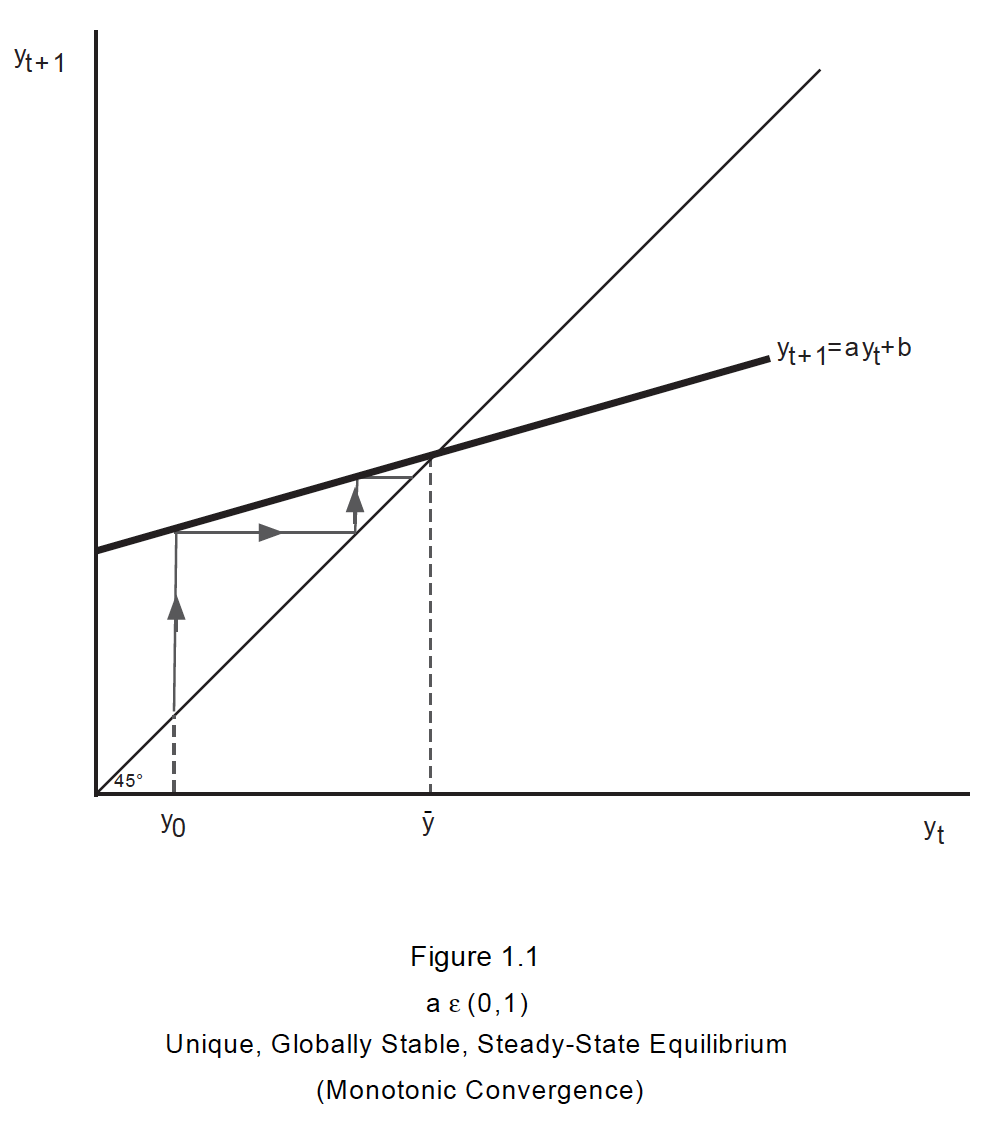
\includegraphics[width = 0.6\textwidth]{./images/fig1}
\end{figure}}
\end{frame}

%%%%%%%%%%%%%%%%%%%%%%%
%%%%%%%% FRAME %%%%%%%%
%%%%%%%%%%%%%%%%%%%%%%%

\begin{frame}
\frametitle{Unique, globally stable SS}
{\begin{figure}
\centering
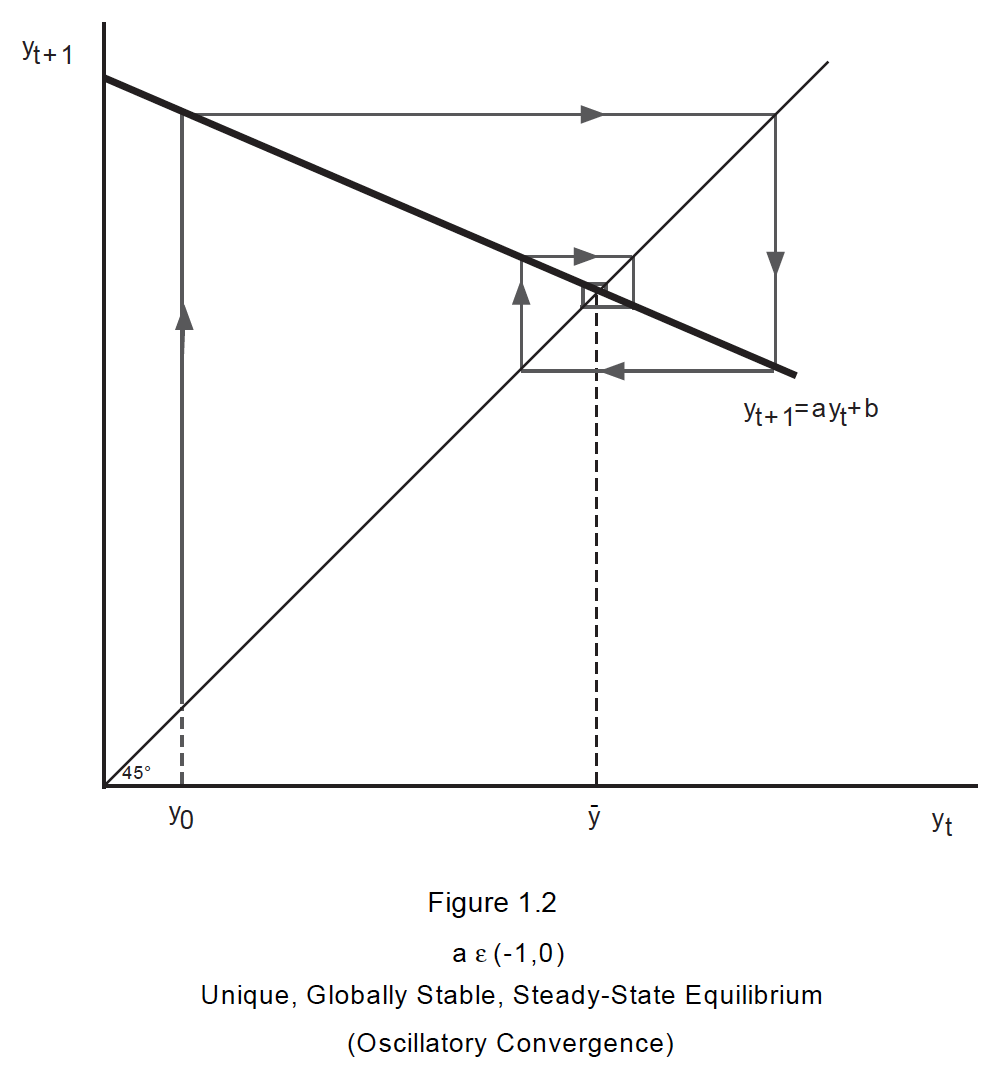
\includegraphics[width = 0.7\textwidth]{./images/fig2}
\end{figure}}
\end{frame}

%%%%%%%%%%%%%%%%%%%%%%%
%%%%%%%% FRAME %%%%%%%%
%%%%%%%%%%%%%%%%%%%%%%%

\begin{frame}
\frametitle{Continuum of unstable SS}
{\begin{figure}
\centering
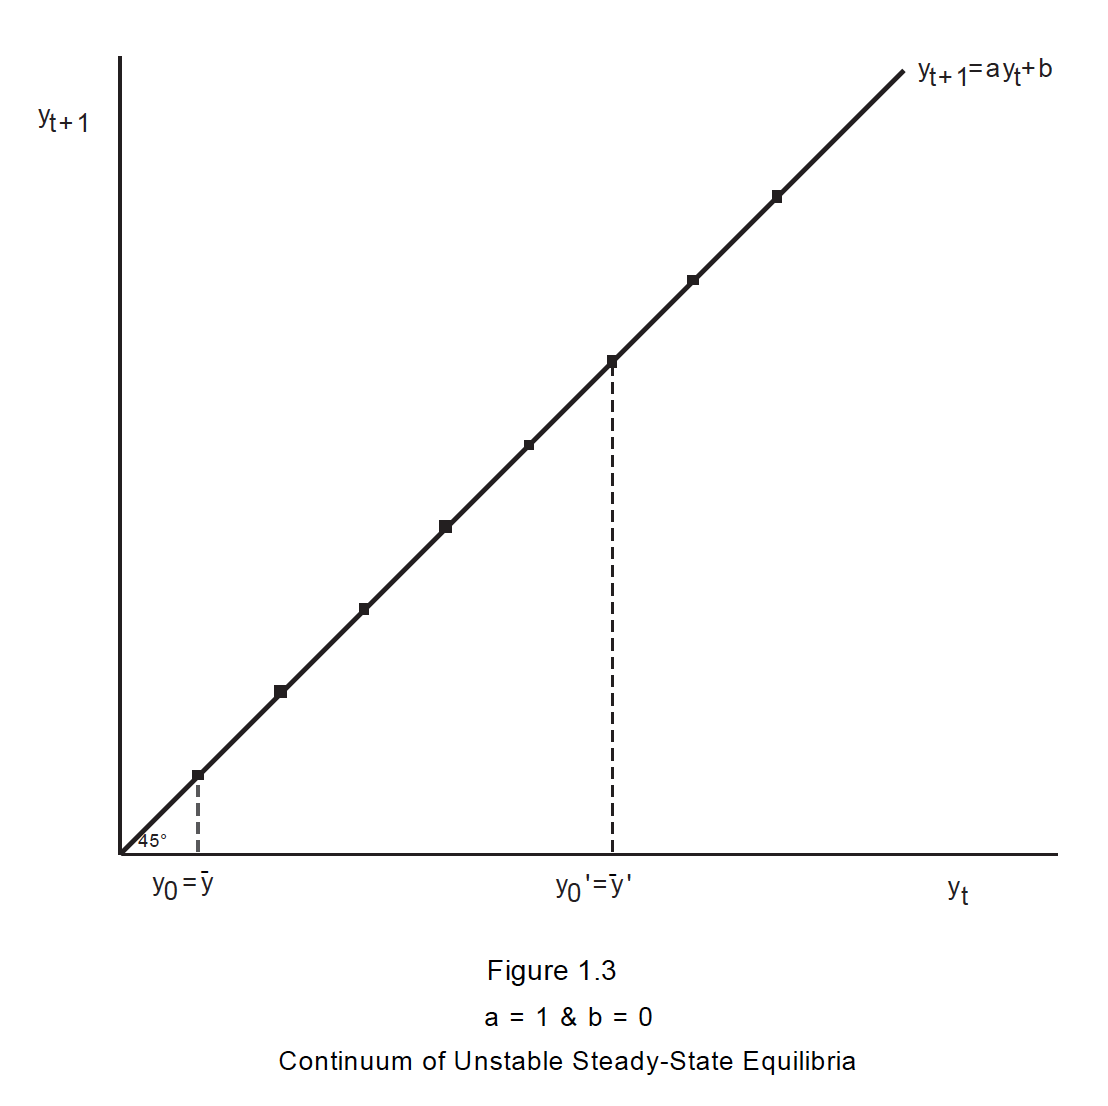
\includegraphics[width = 0.7\textwidth]{./images/fig3}
\end{figure}}
\end{frame}

%%%%%%%%%%%%%%%%%%%%%%%
%%%%%%%% FRAME %%%%%%%%
%%%%%%%%%%%%%%%%%%%%%%%

\begin{frame}
\frametitle{Non-existence of a SS}
{\begin{figure}
\centering
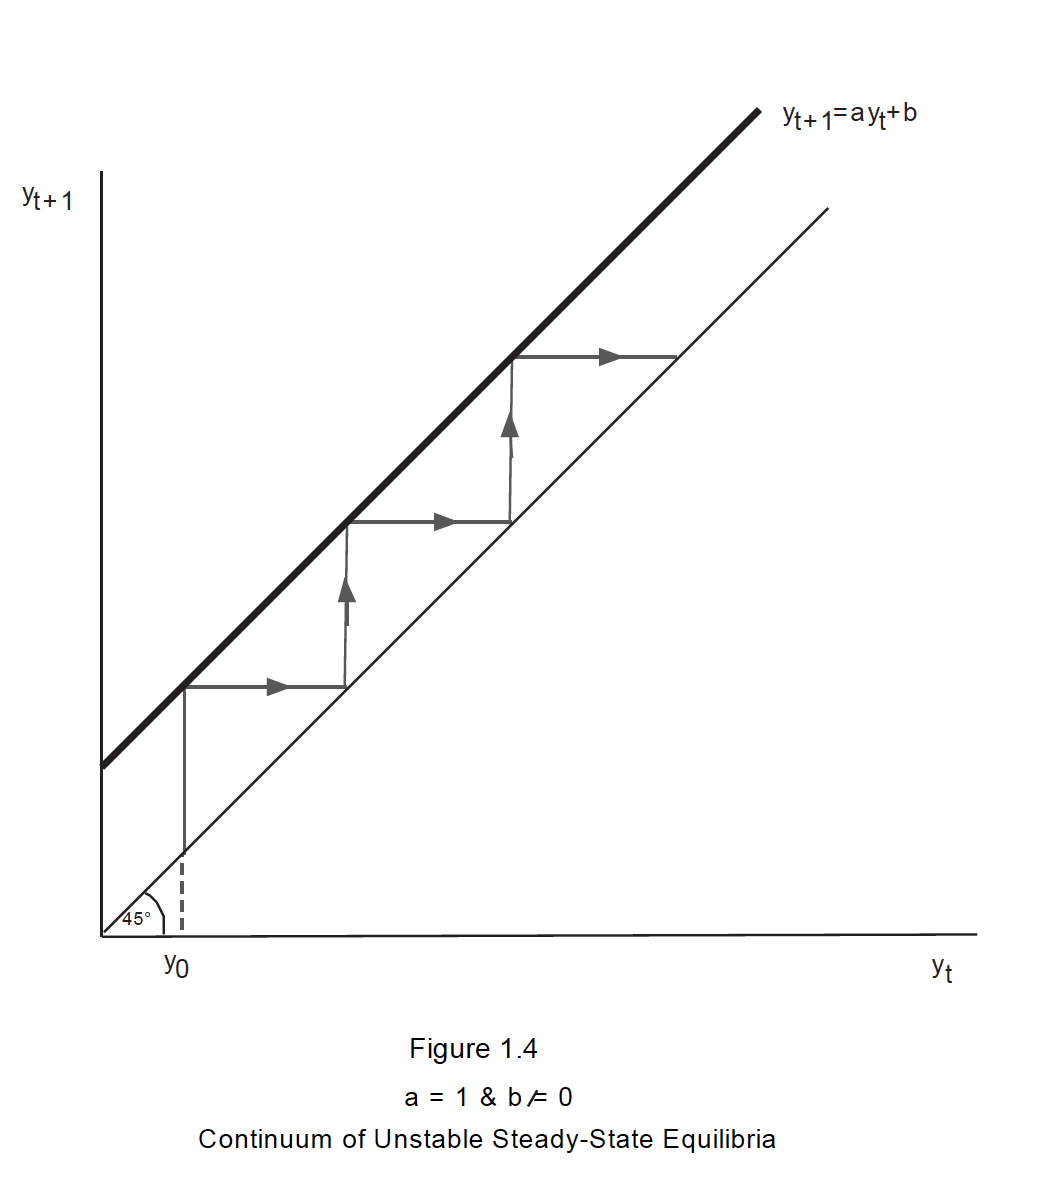
\includegraphics[width = 0.66\textwidth]{./images/fig4}
\end{figure}}
\end{frame}

%%%%%%%%%%%%%%%%%%%%%%%
%%%%%%%% FRAME %%%%%%%%
%%%%%%%%%%%%%%%%%%%%%%%

\begin{frame}
\frametitle{Unique unstable SS}
{\begin{figure}
\centering
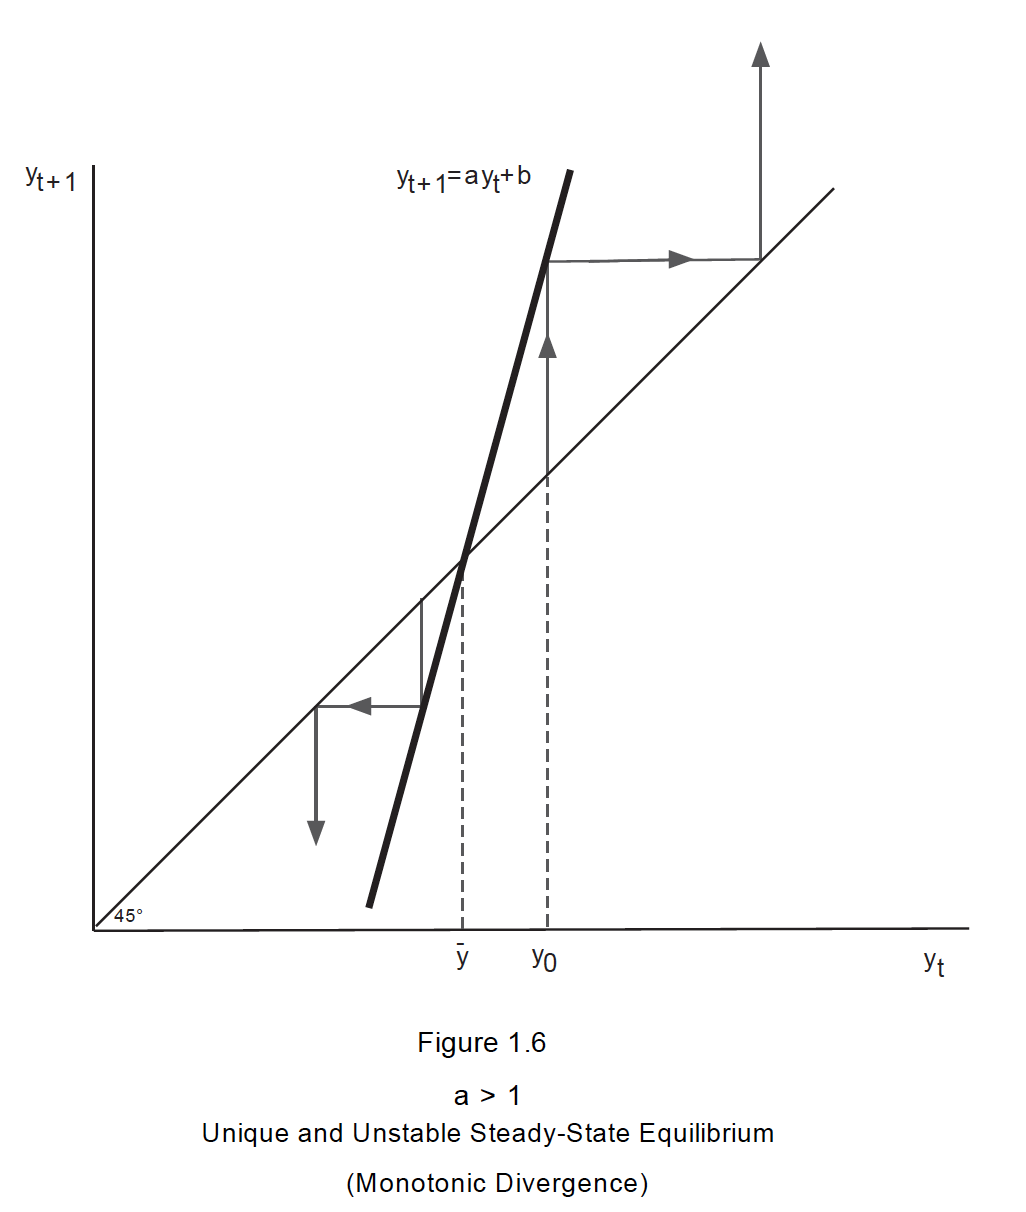
\includegraphics[width = 0.6\textwidth]{./images/fig5}
\end{figure}}
\end{frame}

%%%%%%%%%%%%%%%%%%%%%%%
%%%%%%%% FRAME %%%%%%%%
%%%%%%%%%%%%%%%%%%%%%%%

\begin{frame}
\frametitle{Necessary and Sufficient Condition for Global Stability}
\begin{itemize}\itemsep2ex
	\item Hence the whole discussion leads us to the main stability result:
	\item A steady-state equilibrium of the difference equation $y_{t+1} = a y_t + b$ is \textbf{globally} stable \textbf{if and only if} $|a|<1$.
\end{itemize}
\end{frame}

%%%%%%%%%%%%%%%%%%%%%%%
%%%%%%%% FRAME %%%%%%%%
%%%%%%%%%%%%%%%%%%%%%%%

\begin{frame}
\frametitle{Non-linear systems and solution}
\begin{itemize}\itemsep2ex
	\item We will study the evolution of the state variable \textit{in the proximity} of a SS. Then give sufficient conditions for stability. Consider the one-dimensional first-order state variable
	\begin{equation*}
	y_{t+1} =f (y_t)
	\end{equation*}
	\item Again we use the method of iterations to describe the trajectory of the state variable
	\begin{equation*}
	y_{1} =f (y_0) \implies y_{2} =f (f(y_0)) \equiv f^2(y_0) \implies y_t = f^t(y_0)
	\end{equation*}
	\item Unlike the solution to the linear system, the solution for the nonlinear system is not very informative about the factors of convergence
	\item Hence additional methods of analysis are required (linear approximation around the SS).
\end{itemize}
\end{frame}

%%%%%%%%%%%%%%%%%%%%%%%
%%%%%%%% FRAME %%%%%%%%
%%%%%%%%%%%%%%%%%%%%%%%

\begin{frame}
\frametitle{Steady-State and Linearization}
\begin{itemize}\itemsep2ex
	\item A SS of the difference equation $y_{t+1} =f (y_t) $ is a level of $\bar{y}$ such that $\bar{y} = f(\bar{y})$.  Generically, a non-linear may be characterized by unique SS, multiple SS, chaotic behavior, or non-existence of SS
	\item Consider a first orderTaylor expansion of $y_{t+1}=f (y_t)$ around the SS
	\begin{equation*}
	y_{t+1} =f (\bar{y}) + f'(\bar{y}) (y_t - \bar{y}) = f'(\bar{y}) y_t + f (\bar{y}) - f'(\bar{y}) \bar{y} = ay_t + b
	\end{equation*}
where $a=f'(\bar{y})$ and $b=f (\bar{y}) - f'(\bar{y}) \bar{y}$ are given constants.
	\item Now, simply apply the main result we have learnt for linear systems! However we go for global to local because of the linearization
	\item The SS $\bar{y}$ is \textbf{locally} stable iff $|f'(\bar{y})|<1$.
	\begin{itemize}\itemsep2ex
		\item This is the result used in the Solow model, plus fundamental theorem of calculus to obtain global stability. See proof of proposition 2.5 in Acemoglu
	\end{itemize}
\end{itemize}
\end{frame}

%%%%%%%%%%%%%%%%%%%%%%%
%%%%%%%% FRAME %%%%%%%%
%%%%%%%%%%%%%%%%%%%%%%%

\begin{frame}
\frametitle{Unique globally stable SS}
{\begin{figure}
\centering
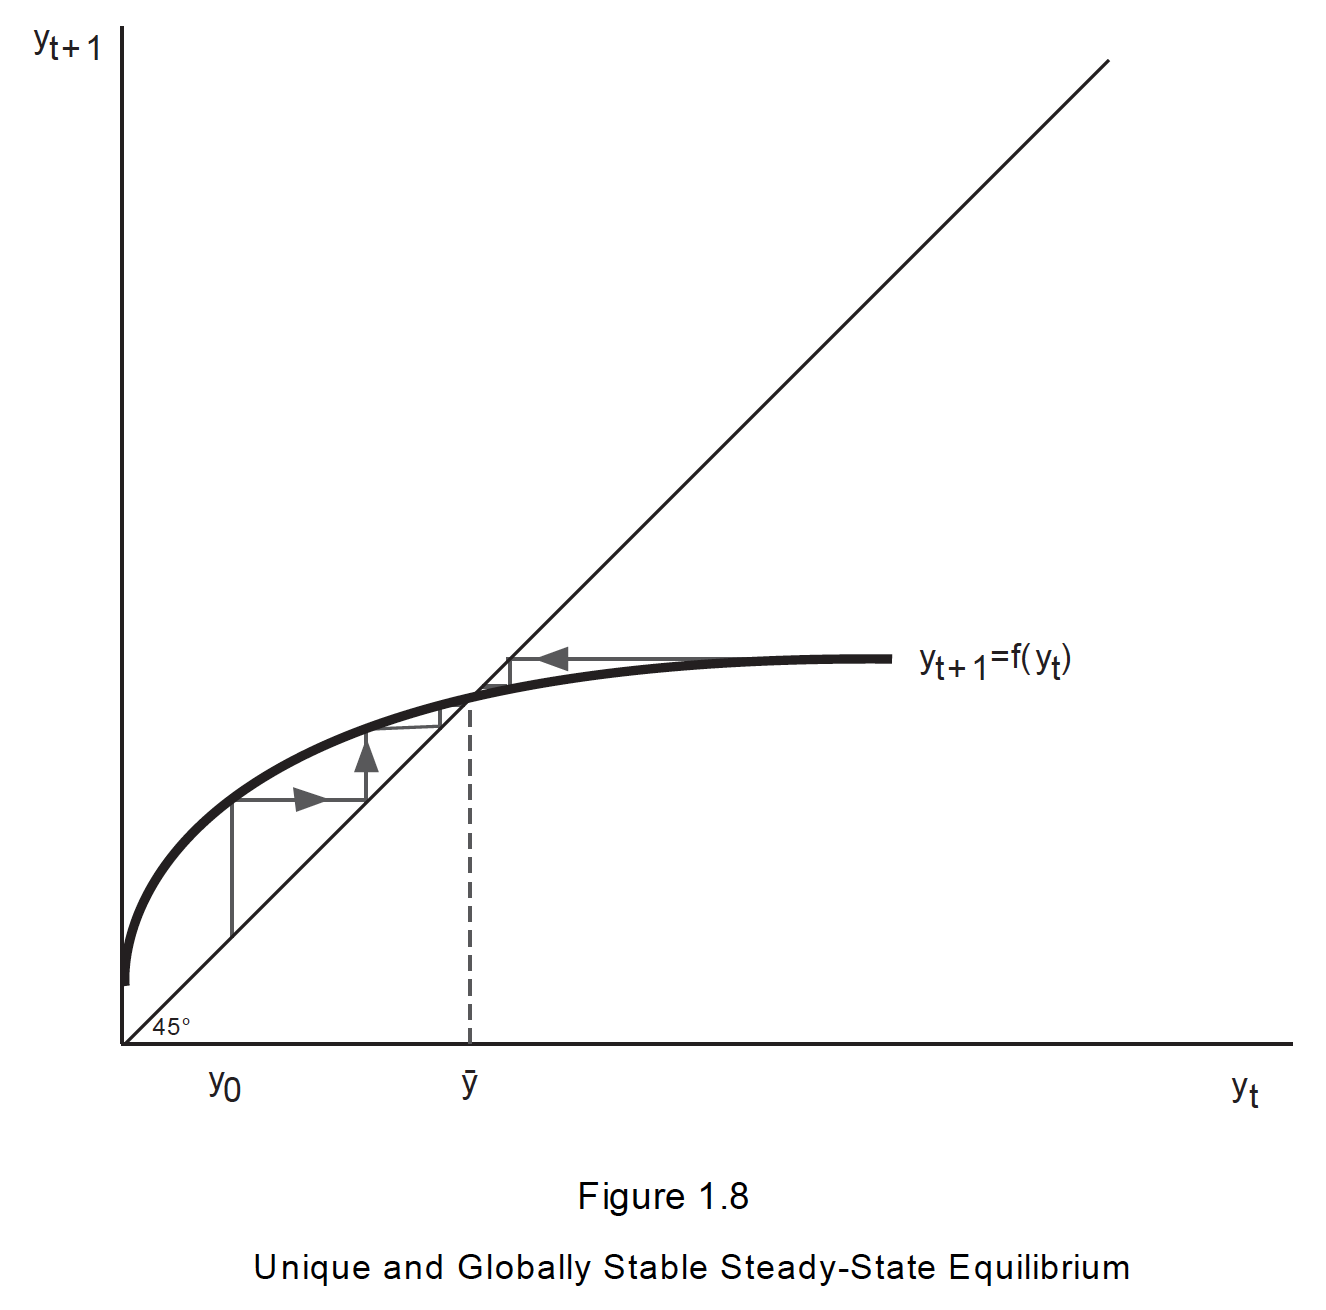
\includegraphics[width = 0.7\textwidth]{./images/fig6}
\end{figure}}
\end{frame}

%%%%%%%%%%%%%%%%%%%%%%%
%%%%%%%% FRAME %%%%%%%%
%%%%%%%%%%%%%%%%%%%%%%%

\begin{frame}
\frametitle{Multiple SS}
{\begin{figure}
\centering
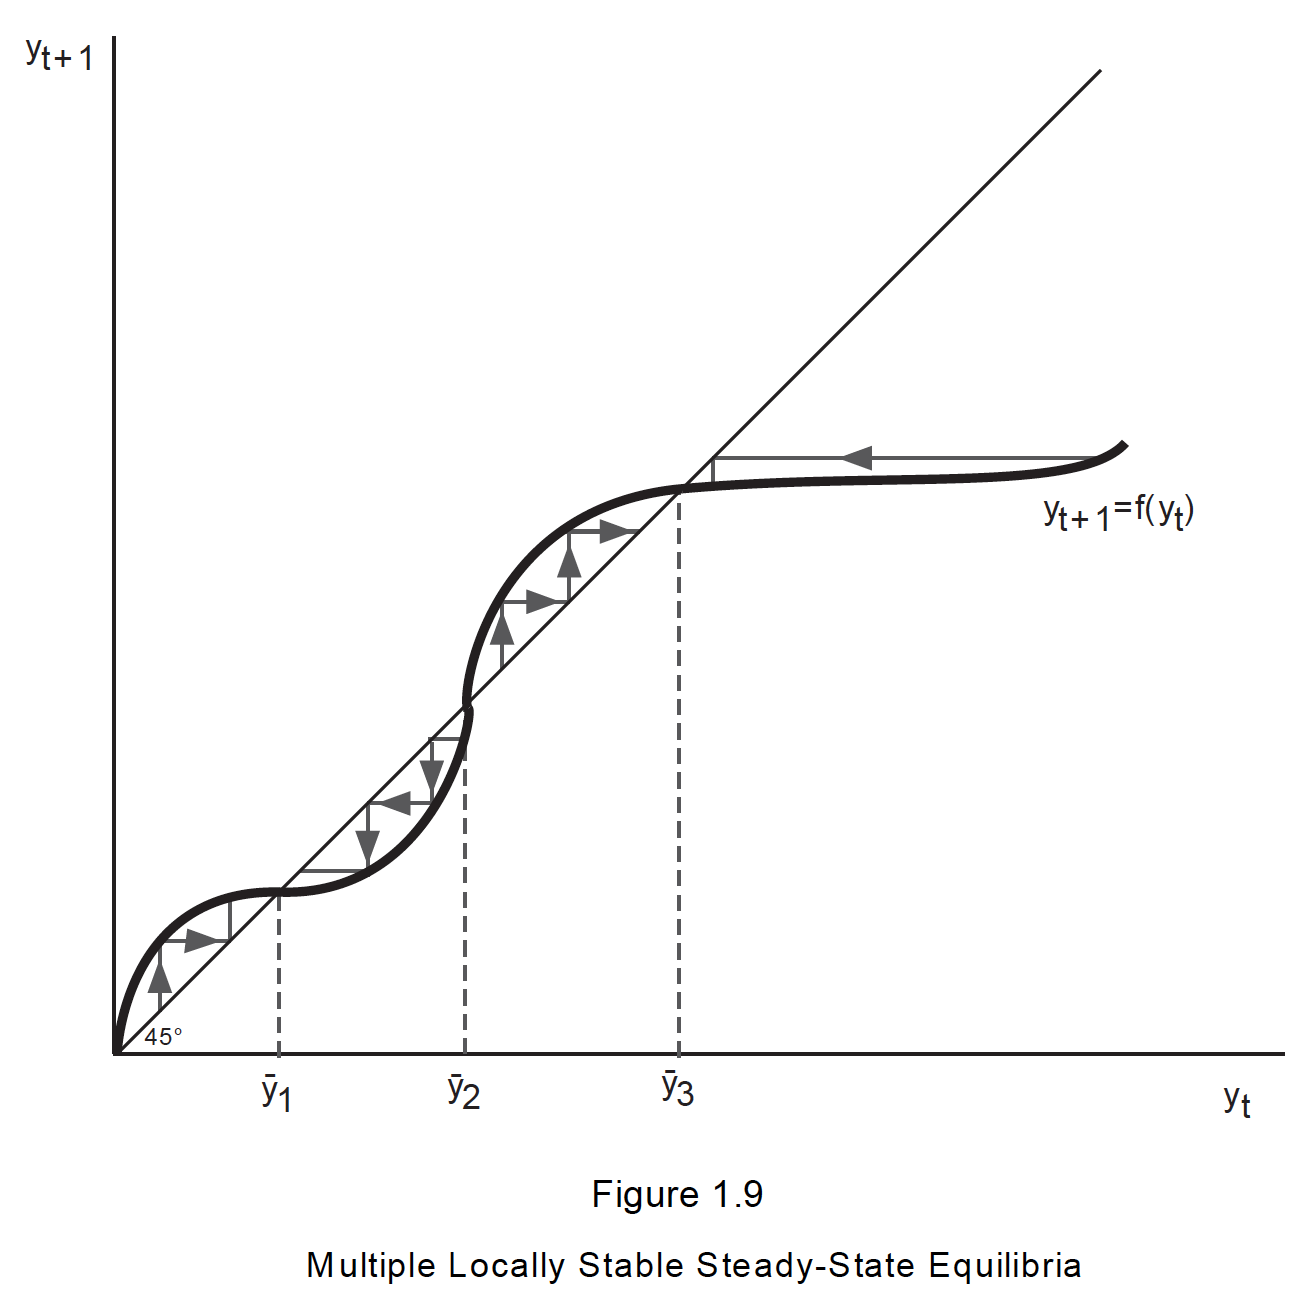
\includegraphics[width = 0.7\textwidth]{./images/fig7}
\end{figure}}
\end{frame}

%%%%%%%%%%%%%%%%%%%%%%%
%%%%%%%% FRAME %%%%%%%%
%%%%%%%%%%%%%%%%%%%%%%%

\begin{frame}
\frametitle{Higher-order Systems (Acemoglu page 44-45)}
\begin{itemize}\itemsep2ex
	\item \textbf{Stability for Systems of Linear Difference Equations}: Consider $x_{t+1} = A x_{t} + b$, where $x$ and $b$ are vectors and $A$ a matrix. Suppose that all of the eigenvalues of A are strictly \textit{inside the unit circle} in the complex plane. Then the SS of the difference equation is globally asymptotically stable.
	\item \textbf{Local Stability for Systems of Non-Linear Difference Equations}: Consider $x_{t+1} = G(x_t)$, where $x$ is a vector and $G$ a non-linear function differentiable at $x^*$. Define $A \equiv D G(x^*)$, where $D G$ denotes the matrix of partial derivatives of $G$. Suppose that all of the eigenvalues of A are strictly \textit{inside the unit circle}. Then the SS of the difference equation is locally stable (there exists an open ball where the trajectory converges).
\end{itemize}
\end{frame}























%%%%%%%%%%%%%%%%%%%%%
%%%%%%%% END %%%%%%%%
%%%%%%%%%%%%%%%%%%%%%

\end{document}


%%%%%%%%%%%%%%%%%%%%%%%
%%%%%%%% FRAME %%%%%%%%
%%%%%%%%%%%%%%%%%%%%%%%

\begin{frame}

	\frametitle{Solving a Linear DE (General Case)}

		\begin{itemize}\itemsep2ex

			\item Start from

\begin{equation*}
\dot{x(t)} = a(t) x(t) + b(t)
\end{equation*}

			\item Rewrite it as $\dot{x(t)} - a(t) x(t) = b(t)$ and multiply both sides by $\exp ( - \int_0^t a(s) ds)$

			\item Integrate both sides and divide them by $\exp ( - \int_0^t a(s) ds)$ to obtain


\begin{equation*}
x(t) = \left [c + \int_0^t b(s)  \left ( \exp \int_0^s a(v) dv \right )^{-1} ds \right ] \exp \left( \int_0^t a(s) ds \right )
\end{equation*}


		\end{itemize}

\end{frame}
